\section{Implementation of Essence}
%todo A description of use context and selected use scenarios (see Essence-book Chapter 13).

%todo A discussion of how to implement support for key use scenarios (see Essence-book Chapter 14).

\subsection{Use context}
According to \cite[ p. 83]{essence} the definition of an use context is:

\begin{center}
	“\textit{Use context} - the physical, legal, and systemic world, where the scenario unfolds.
	 The locations, physical constraints, rules, regulations, preexisting systems, and technological platforms relevant to the design process.”
\end{center}

The use context for our project is a world where smartphones are used while running.
In this world people listen to music while running, through their smartphones.
Smartphones have built in accelerometer, GPS, internet access, etc..
Runners have their smartphones attached to their arms, limiting the view of the smartphones' screens.
The runners use headphones specialised for running, ensuring they can still hear the traffic while listening to music.

Running can take place both outdoor and indoor on a treadmill.
Indoor running limits some technological sensors, e.g. GPS, but enhances other features such as internet access through WiFi.
Outdoor running can in some places restrict the internet access, but enables the use of other sensors such as GPS.

Supplementary sensors can be accessed through other technological devices such as wearables.
Especially smartwatches are a popular and useful addition to the smartphone.

A lot of services are available through the internet.
Some of these services include beats-per-minute lookup for songs, streaming of music, and other information related to music.


\subsection{Use Scenarios}
Given the previously defined use context, there exists several use scenarios.
Here is a sample of use scenarios:

\begin{itemize}
	\item When the application is started, it searches predefined directories for new music and adds it to the collection.
	\item The music starts playing when the runner starts running.
	\item When the runner stops running for more than a minute, the music stops playing.
	\item If the runner only stops for less than a minute, the music only pauses.
	\item While the runner is running, if he mildly changes his pace, the music will adjust its tempo.
	\item If he instead changes his pace drastically, the song will change.
	\item While running he/she can tap the screen of the smartphone on his arm to control the music.
	\item A song does not have an associated BPM value. The phone calculates, and uploads it to a server.
\end{itemize}

The use cases and actors can be seen in \Cref{fig:useCase}.

\begin{figure}[h!]
  \centering
    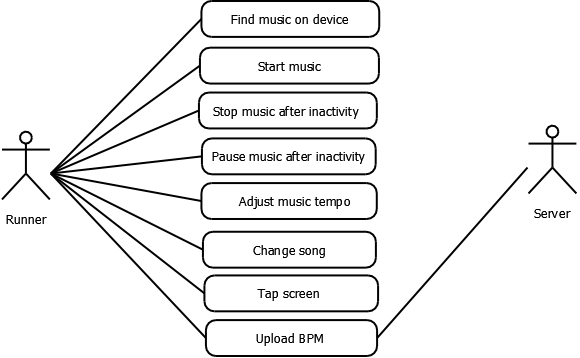
\includegraphics[width=\textwidth]{Images/useCase.png}
    \caption{A use case diagram of some of the use scenarios}
    \label{fig:useCase}
\end{figure}

%todo A discussion of how to implement support for key use scenarios (see Essence-book Chapter 14).
\subsection{Implementation Discussion}
We will now discuss how the different use scenarios can be implemented in the current use context.
\begin{itemize}
	\item It is possible to use a listener to detect when the application starts. When this is detected, a depth-first-search algorithm can be run with start in a predefined directory. If the search finds any new music, it can be added to the collection.
	
	\item Given the application runs on a modern smartphone, it is possible to access data from an accelerometer. Based on this data, we can calculate when the runner starts running. When this happens the application can start the music.
	
	We will use the accelerometer instead of GPS, because the accelerometer is accessible in both indoor and outdoor environments. Further if the runner used a treadmill, the movement will not be showing on the GPS.
	
	\item By using the accelerometer it is also possible to detect when the runner is standing still. We can then start a timer, then depending on the time since standstill, we can either stop the music or pause it.
	
	\item The accelerometer can, hence the name, detect changes in acceleration.
	This can be used to determine if the runner changes his pace, and of what magnitude the change is.
	Based on this information, we can adjust the tempo of the music or we can change song if needed.
	
	\item Utilising the screen listeners will allow for detecting taps, even though the screen is off.
	
	\item An algorithm can be used to calculate a BPM value for a song which does not have an associated BPM value. It can then be uploaded to a server for future use by others. 
\end{itemize}
